% Created by tikzDevice version 0.8.1 on 2015-11-06 00:42:54
% !TEX encoding = UTF-8 Unicode
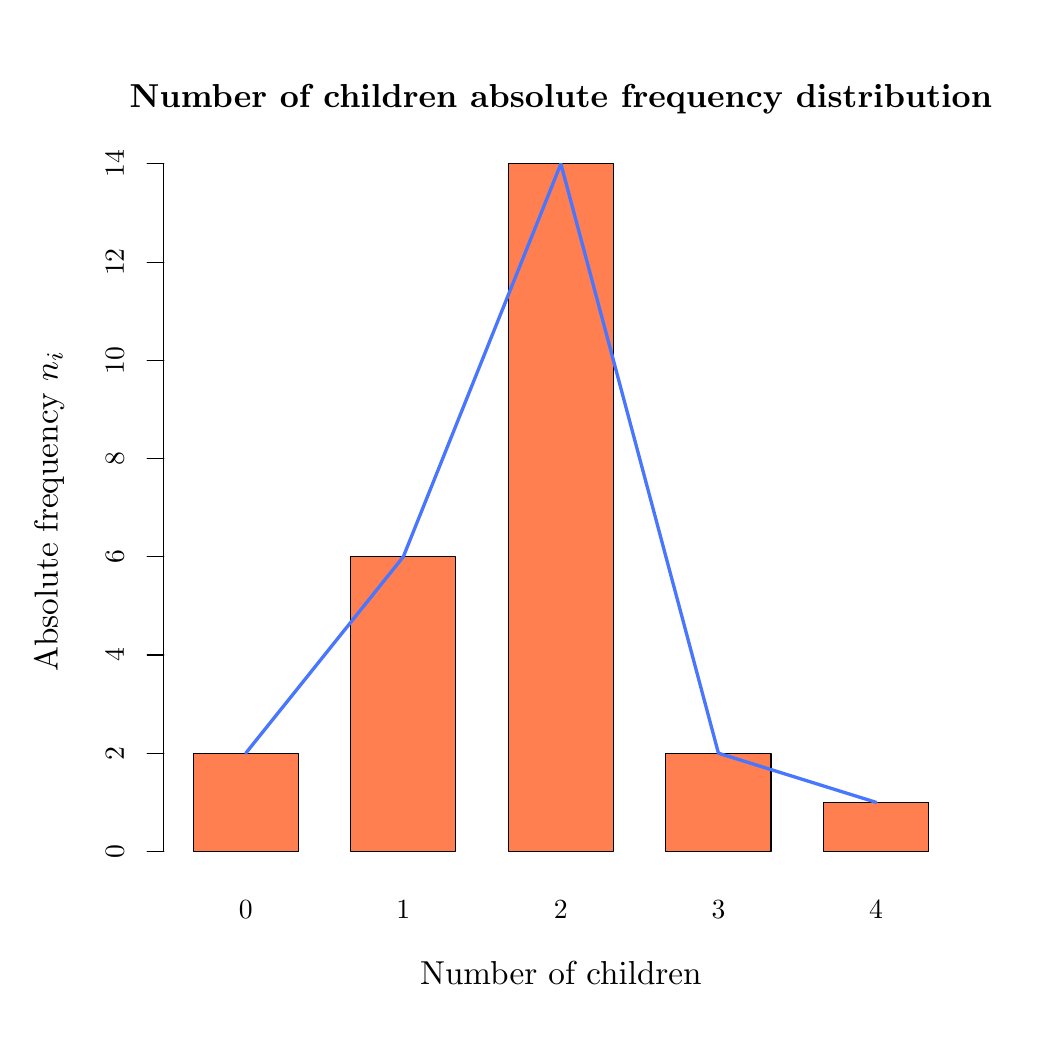
\begin{tikzpicture}[x=1pt,y=1pt]
\definecolor{fillColor}{RGB}{255,255,255}
\path[use as bounding box,fill=fillColor,fill opacity=0.00] (0,0) rectangle (361.35,361.35);
\begin{scope}
\path[clip] (  0.00,  0.00) rectangle (361.35,361.35);
\definecolor{drawColor}{RGB}{0,0,0}
\definecolor{fillColor}{RGB}{255,127,80}

\path[draw=drawColor,line width= 0.4pt,line join=round,line cap=round,fill=fillColor] ( 59.83, 63.68) rectangle ( 97.78, 99.18);

\path[draw=drawColor,line width= 0.4pt,line join=round,line cap=round,fill=fillColor] (116.76, 63.68) rectangle (154.72,170.17);

\path[draw=drawColor,line width= 0.4pt,line join=round,line cap=round,fill=fillColor] (173.70, 63.68) rectangle (211.65,312.15);

\path[draw=drawColor,line width= 0.4pt,line join=round,line cap=round,fill=fillColor] (230.63, 63.68) rectangle (268.59, 99.18);

\path[draw=drawColor,line width= 0.4pt,line join=round,line cap=round,fill=fillColor] (287.57, 63.68) rectangle (325.52, 81.43);
\end{scope}
\begin{scope}
\path[clip] (  0.00,  0.00) rectangle (361.35,361.35);
\definecolor{drawColor}{RGB}{0,0,0}

\node[text=drawColor,anchor=base,inner sep=0pt, outer sep=0pt, scale=  1.00] at ( 78.81, 39.60) {0};

\node[text=drawColor,anchor=base,inner sep=0pt, outer sep=0pt, scale=  1.00] at (135.74, 39.60) {1};

\node[text=drawColor,anchor=base,inner sep=0pt, outer sep=0pt, scale=  1.00] at (192.67, 39.60) {2};

\node[text=drawColor,anchor=base,inner sep=0pt, outer sep=0pt, scale=  1.00] at (249.61, 39.60) {3};

\node[text=drawColor,anchor=base,inner sep=0pt, outer sep=0pt, scale=  1.00] at (306.54, 39.60) {4};
\end{scope}
\begin{scope}
\path[clip] (  0.00,  0.00) rectangle (361.35,361.35);
\definecolor{drawColor}{RGB}{0,0,0}

\node[text=drawColor,anchor=base,inner sep=0pt, outer sep=0pt, scale=  1.20] at (192.68,332.61) {\bfseries Number of children absolute frequency distribution};

\node[text=drawColor,anchor=base,inner sep=0pt, outer sep=0pt, scale=  1.20] at (192.68, 15.60) {Number of children};

\node[text=drawColor,rotate= 90.00,anchor=base,inner sep=0pt, outer sep=0pt, scale=  1.20] at ( 10.80,186.67) {Absolute frequency $n_i$};
\end{scope}
\begin{scope}
\path[clip] (  0.00,  0.00) rectangle (361.35,361.35);
\definecolor{drawColor}{RGB}{0,0,0}

\path[draw=drawColor,line width= 0.4pt,line join=round,line cap=round] ( 49.20, 63.68) -- ( 49.20,312.15);

\path[draw=drawColor,line width= 0.4pt,line join=round,line cap=round] ( 49.20, 63.68) -- ( 43.20, 63.68);

\path[draw=drawColor,line width= 0.4pt,line join=round,line cap=round] ( 49.20, 99.18) -- ( 43.20, 99.18);

\path[draw=drawColor,line width= 0.4pt,line join=round,line cap=round] ( 49.20,134.67) -- ( 43.20,134.67);

\path[draw=drawColor,line width= 0.4pt,line join=round,line cap=round] ( 49.20,170.17) -- ( 43.20,170.17);

\path[draw=drawColor,line width= 0.4pt,line join=round,line cap=round] ( 49.20,205.66) -- ( 43.20,205.66);

\path[draw=drawColor,line width= 0.4pt,line join=round,line cap=round] ( 49.20,241.16) -- ( 43.20,241.16);

\path[draw=drawColor,line width= 0.4pt,line join=round,line cap=round] ( 49.20,276.65) -- ( 43.20,276.65);

\path[draw=drawColor,line width= 0.4pt,line join=round,line cap=round] ( 49.20,312.15) -- ( 43.20,312.15);

\node[text=drawColor,rotate= 90.00,anchor=base,inner sep=0pt, outer sep=0pt, scale=  1.00] at ( 34.80, 63.68) {0};

\node[text=drawColor,rotate= 90.00,anchor=base,inner sep=0pt, outer sep=0pt, scale=  1.00] at ( 34.80, 99.18) {2};

\node[text=drawColor,rotate= 90.00,anchor=base,inner sep=0pt, outer sep=0pt, scale=  1.00] at ( 34.80,134.67) {4};

\node[text=drawColor,rotate= 90.00,anchor=base,inner sep=0pt, outer sep=0pt, scale=  1.00] at ( 34.80,170.17) {6};

\node[text=drawColor,rotate= 90.00,anchor=base,inner sep=0pt, outer sep=0pt, scale=  1.00] at ( 34.80,205.66) {8};

\node[text=drawColor,rotate= 90.00,anchor=base,inner sep=0pt, outer sep=0pt, scale=  1.00] at ( 34.80,241.16) {10};

\node[text=drawColor,rotate= 90.00,anchor=base,inner sep=0pt, outer sep=0pt, scale=  1.00] at ( 34.80,276.65) {12};

\node[text=drawColor,rotate= 90.00,anchor=base,inner sep=0pt, outer sep=0pt, scale=  1.00] at ( 34.80,312.15) {14};
\end{scope}
\begin{scope}
\path[clip] ( 49.20, 61.20) rectangle (336.15,312.15);
\definecolor{drawColor}{RGB}{72,118,255}

\path[draw=drawColor,line width= 1.2pt,line join=round,line cap=round] ( 78.81, 99.18) --
	(135.74,170.17) --
	(192.67,312.15) --
	(249.61, 99.18) --
	(306.54, 81.43);
\end{scope}
\end{tikzpicture}
